\documentclass[10pt,letterpaper]{article} 
\usepackage{tikz}
\usepackage{toolsper}
%\usepackage{graphicx}‎‎
%\usefonttheme{serif}‎
%\usepackage{ptext}‎
%\usepackage{xepersian}
%\settextfont{B Nazanin}
\usepackage{lipsum}
\setlength{\parindent}{0pt}
%\usepackage{enumitem}
%\setlist[enumerate,1]{label=(\arabic*)}
\newcommand{\pf}{$\blacksquare$}
\newcommand{\EX}{\Bbb E}
\newcommand{\nl}{\newline\newline}
\setlength{\parskip}{1em}

\usepackage{amsmath}
\usepackage{accents}
\newlength{\dhatheight}
\newcommand{\doublehat}[1]{%
    \settoheight{\dhatheight}{\ensuremath{\hat{#1}}}%
    \addtolength{\dhatheight}{-0.35ex}%
    \hat{\vphantom{\rule{1pt}{\dhatheight}}%
    \smash{\hat{#1}}}}

\newcounter{QuestionNumber}
\setcounter{QuestionNumber}{1}

\newcommand{\Q}{
\textbf{
سوال \theQuestionNumber)
}
\stepcounter{QuestionNumber}
}

\newcommand{\fig}[3]{
\begin{figure}[h!]
#1
\caption{#2}
\label{#3}
\end{figure}
}

\newcommand{\subfig}[3]{
\begin{subfigure}{#3}
#1
\caption{#2}
\end{subfigure}
}
%\newcommand{\pic}[2]{
%\begin{center}
%\includegraphics[width=#2]{#1}
%\end{center}
%}
\begin{document}
\Large
\begin{center}
به نام زیبایی

تمرینات سری دوازدهم سیگنال ها و سیستم ها
\hl
\end{center}
\Q

تبدیل z هر یک از سیگنال های زیر را به همراه ناحیه همگرایی آن به دست آورید. در هر مورد استدلال کنید آیا سیگنال تبدیل فوریه دارد یا خیر.

الف)
$
x[n]=\delta[n-1]+2\delta[n-2]
$

ب)
$
x[n]=(-1)^nu[n]
$

پ)
$
x[n]=({1\over 3})^{n-2}u[n-2]
$

\Q

برای هر یک تبدیل z های زیر با ناحیه همگرایی داده شده، سیگنال حوزه زمان را بیابید (برای تجزیه کسرها از روش تجزیه به کسرهای جزئی بهره بگیرید).

الف)
$
X(z)={2-z^{-1}\over 1-{1\over 4}z^{-2}}\quad,\quad |z|>{1\over 2}
$

ب)
$
X(z)={z^{-1}-{1\over 2}\over (1-{1\over 2}z^{-1})^2}\quad,\quad |z|<{1\over 2}
$

پ) 
$
X(z)={3\over z-{1\over 4}-{1\over 8}z^{-1}}
$
 و ناحیه همگرایی به گونه ای است که سیگنال حوزه زمان، تبدیل فوریه دارد.
%\newline

\Q
در هر یک از نمودارهای صفر-قطب زیر، اندازه پاسخ فرکانسی (تبدیل فوریه) سیگنال را به  صورت تقریبی و به روش هندسی رسم کنید (نیازی به تعیین محل دقیق قطب ها و صفرها نیست؛ فقط نمودار تقریبی مد نظر است).

\begin{figure}[h!]
\centering
\begin{subfigure}{0.49\textwidth}
\includegraphics[width=77mm]{PS12_Q3_3.eps}
\caption{}
\end{subfigure}
\begin{subfigure}{0.49\textwidth}
\includegraphics[width=77mm]{PS12_Q3_4.eps}
\caption{}
\end{subfigure}
\end{figure}
\begin{figure}
\ContinuedFloat
\centering
%%%%%%%%%%%%
\begin{subfigure}{0.49\textwidth}
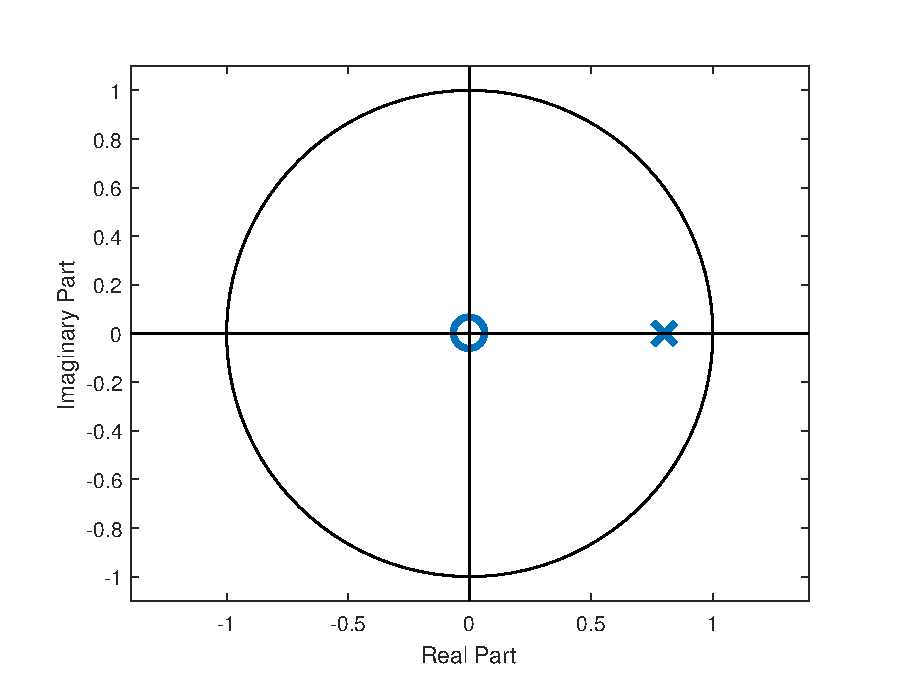
\includegraphics[width=77mm]{PS12_Q3_1.eps}
\caption{}
\end{subfigure}
%%%%%%%%%%%%
\begin{subfigure}{0.49\textwidth}
\includegraphics[width=77mm]{PS12_Q3_2.eps}
\caption{}
\end{subfigure}
%%%%%%%%%%%%
\end{figure}
%\Qچ نمودار صفر-قطب زیر، 

\Q

فرض کنید اطلاعات زیر در مورد یک سیگنال گسسته $x[n]$ داده شده است:

1. $x[n]$
 حقیقی و دست راستی است.

2. $X(z)$
 دقیقا دو قطب دارد.

3. $X(z)$
یک صفر مرتبه 2 در صفر دارد.

4. $X(z)$
 یک قطب در 
$
{1\over 2}e^{j{\pi\over 3}}
$
 دارد.

5. $X(1)={8\over 3}$

در این صورت، 
$
X(z)
$
 و ناحیه همگرایی آن را به دست آورید.

\Q

فرض کنید اطلاعات زیر در مورد یک سیستم LTI داده شده است:

1. پاسخ سیستم به ورودی 
$
x[n]=(-2)^n
$
برابر 
$
y[n]=0
$
است.

2. پاسخ سیستم به ورودی 
$
x[n]=({1\over 2})^nu[n]
$
، به فرم
$$
y[n]=\delta[n]+a({1\over 4})^nu[n]
$$
است که 
$
a
$
 یک ثابت است.

الف) مقدار $a$ را بیابید.

ب) پاسخ این سیستم را به ورودی 
$
x[n]=1
$
 بیابید.

پ) پاسخ این سیستم را به ورودی 
$
x[n]=\left(-{1\over 6}\right)^n
$
 بیابید.

\Q

نمودار صفر-قطب پاسخ ضربه‌ی دو سیستم گسسته‌ (سیستم 1 با پاسخ ضربه‌ی 
$
h_1[n]
$
و سیستم 2 با پاسخ ضربه‌ی 
$
h_2[n]
$
)
 به صورت زیر است:
\begin{figure}[h!]
\centering
\begin{subfigure}{0.49\textwidth}
\includegraphics[width=70mm]{PS12_Q3_6.eps}
\caption{
نمودار صفر-قطب سیستم 1؛ این سیستم دارای دو قطب در $0.8$ و $1.2$ و دو صفر در $0.3$ و $-1$ است.
}
\end{subfigure}
\begin{subfigure}{0.49\textwidth}
\includegraphics[width=70mm]{PS12_Q3_5.eps}
\caption{
نمودار صفر-قطب سیستم 2
}
\end{subfigure}
\end{figure}

سیستم 1 پایدار و سیستم 2 علی است.

الف) آیا سیستم 1 علی است؟ دوطرفه چطور؟

ب) آیا سیستم 2 پایدار است؟

پ) پاسخ فرکانسی سیستم 1 ($H_1(e^{j\omega})$) در کدام فرکانس صفر می شود؟

ت) با رسم تقریبی اندازه‌ی پاسخ فرکانسی سیستم 1 ($|H_1(e^{j\omega})|$) استدلال کنید این سیستم فیلتر بالاگذر است یا میان گذر یا پایین گذر.

ث) نمودار صفر-قطب تبدیل z سیستم معکوس سیستم 1 را رسم و ناحیه همگرایی آن را تعیین کنید.

\Q

خواص تبدیل z را اثبات کنید!

اگر 
$
x[n]
$
 سیگنالی با تبدیل 
$
X(z)
$
 و ناحیه همگرایی $R$ باشد، نشان دهید (در هر مورد، ناحیه همگرایی تبدیل z سیگنال زمانی را بیابید)

الف)
$$
a^nx[n]\iff X(a^{-1}z)
$$
ب)
$$
x[n]\iff X^*(z^*)
$$
پ)
$$
x[-n]\iff X(z^{-1})
$$
ت)
$$
nx[n]\iff -z{d X(z)\over dz}
$$
ث)
$$
\sum_{k=-\infty}^{n}x[k]\iff {X(z)\over 1-z^{-1}}
$$
\end{document}